\documentclass[10pt, a4paper]{awesome-cv}
\geometry{left=1.4cm, top=.8cm, right=1.4cm, bottom=1.8cm, footskip=.5cm}
\fontdir[fonts/]
\usepackage{multicol}
\usepackage{xcolor}% http://ctan.org/pkg/xcolor

\usepackage{datenumber, fp}
\newcounter{birthday}
\newcounter{today}
\setmydatenumber{birthday}{1982}{08}{26}
\setmydatenumber{today}{\the\year}{\the\month}{\the\day}
\FPsub\result{\thetoday}{\thebirthday}
\FPdiv\myage{\result}{365.2425}
\FPtrunc\myage{\myage}{0}

\hypersetup{%
  colorlinks=false,% hyperlinks will be black
  linkbordercolor=red,% hyperlink borders will be red
  pdfborderstyle={/S/U/W 1}% border style will be underline of width 1pt
}

\colorlet{awesome}{awesome-concrete}
% Set false if you don't want to highlight section with awesome color
\setbool{acvSectionColorHighlight}{true}
\renewcommand{\acvHeaderSocialSep}{\quad\textbar\quad}

\name{Glaucio}{Melo}
\position{[Computer Scientist{\enskip\textbar\enskip}Musician]}

\mobile{(+55) 19 992.537.268}
\email{glaucio.melo@gmail.com}
\skype{gm2.glaucio}
\twitter{glauciogmm}
\linkedin{glauciom}
\github{glauciom}

\quote{\myage~years old, Brazilian, Married}

\usepackage{multirow, tabu}
\newcommand{\tableline}{\\ \tabucline{2-5}\multicolumn{1}{c|}{}&}
\newcommand{\ini}{&x&&}
\newcommand{\inter}{&&x&}
\newcommand{\avan}{&&&x}
\newcommand{\nextline}{\\ \tabucline[1pt]{1-5}}
\newcommand{\finalize}{\nextline}
\newcommand{\drawheader}{& & \multicolumn{3}{c}{Proficiency} \\ \tabucline[1pt]{3-5} \multicolumn{1}{ c }{}& & B & I & A\nextline}

\newcommand{\createfirstline}[2]
{
\multicolumn{1}{c|}{\multirow{#2}{*}{#1}} &
}

\newcommand{\createline}[2]
{
\nextline \multicolumn{1}{c|}{\multirow{#2}{*}{#1}} &
}

\newcommand{\createitem}[1]
{
\multicolumn{1}{|c|}{#1}
}
\newcommand{\til}{\~{}}


\begin{document}

\makecvheader
\begin{picture}(0,0)
    \put(445,28){\frame{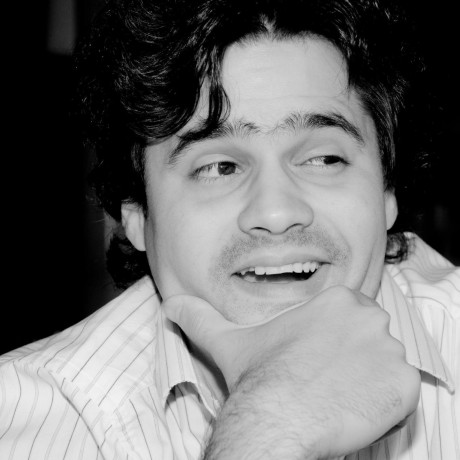
\includegraphics[width=7em]{resume/cv.jpg}}}
\end{picture}

\makecvfooter
  {\today}
  {Glaucio Melo~~~·~~~about.me}
  {\thepage}

 \cvsection{Summary}

\begin{cvparagraph}
I’m a passionate computer programmer with Bachelor’s degree in Computer Science and nearly 18 years 
of practical experience on several IT platforms and programming languages, creating and maintaining 
products / on-demand projects throughout all software life cycle / ecosystems. 
I always do my best about \textbf{everything} I’m committed to accomplish, no matter I’m an expert 
or not on what it has to be done. Between 2006-2013 I owned a small consultancy company 
($[gm]^2$ Intelligent Systems), which was focused mostly on R\&D, machine learning and time series forecasting.
\end{cvparagraph}

 \cvsection{Accomplishments}

\begin{cvparagraph}

Through all these years working with Information Technology, I have acquired experience at 10 different companies, performing several job positions. Most of these experiences were executed in parallel or throughout my overall experience.

\begin{itemize}
\item Currently working as a troubleshooter / full-stack IT specialist, talking to different teams in order to get the things done, applying effective communication. Using AWS/Spring Framework/SQL/NoSQL Databases, dealing with 170 millions (and growing up) requests per day;
\item Third-party team member, being part of HP global contact center migration;
\item Project Lead, responsible for Railroad planning systems implementation from north to south in Chile;
\item $\sim$18 years of overall IT experience, working at several companies with different businesses;
\item $\sim$16 years working with Java Platform (as the main language), from old to new systems;
\item 10+ years of troubleshooting skills in several languages and platforms, from new to legacy systems, as an issues solver;
\item 10+ years working with Ruby  (as an accessory language for automation and quick tasks);
\item $\sim$10 years as a functional language evangelist (mostly with Erlang/OTP and now with Elixir language);
\item $\sim$10 years with front-end development (5 years with desktop programming and 5 years as web developer);
\item 6+ years performing Technical Interviews, nearly 350 candidates for different roles (UX Design, Software Developers, Software Testers, Lead Developers and Software Architects);
\item 6+ years playing Technical Coordination and CTO activities at several different companies;
\item 4+ years as a skilled on-site/remote systems deployer and doing face-to-face meetings with customers and business partners;
\item 4+ years building platforms in JSE/JEE/Spring Framework, directed for parallel / clustered / highly available systems;
\item 3+ years doing Pre-sales, technical coordination and daily conference calls with several countries and several different customers;
\item $\sim$2 years of experience with start-up companies, directed for time series forecasting and alumni social networks.
\end{itemize}
\end{cvparagraph}

 \cvsection{Interests}
\noindent
\vspace{-0.3cm}
\begin{multicols*}{3}
\begin{cventries}
\noindent
\cventry
   {Personal Interests}{}{}{}
   {
     \begin{cvitems}
       \item Music production;
       \item Duathlon (Running / Biking);
       \item Life/work time balance;
       \item Learn new Languages and Cultures;
       \item Continuous improvement on soft skills;
       \item Graphic Novels in general;
       \item Quality of life.
       \end{cvitems}
   }
\end{cventries}
\columnbreak
\begin{cventries}
\noindent
\cventry
    {Professional Interests}{}{}{}
    {
      \begin{cvitems}
        \item Project Management;
        \item Software Engineering;
        \item Systems Architecture;
        \item Research and Development Labs;
        \item Technical Training;
        \item Construction of Custom Softwares;
        \item Technical Interviews;
        \item Big Data;
        \item Data Science.
      \end{cvitems}
    }
\end{cventries}
\columnbreak
\begin{cventries}
\noindent
\cventry
    {Academic Interests}{}{}{}
    {
      \begin{cvitems}
        \item Combinatorial Optimisation;
        \item Machine Learning Techniques;
        \item Swarm Intelligence;
        \item Search Algorithms;
        \item Oil Engineering;
        \item Scheduling Theory;
        \item Digital Image Processing;
        \item Natural Language Processing.
      \end{cvitems}
    }
\end{cventries}
\end{multicols*}













 \cvsection{Technical Knowledge}
~\\
\begin{center}
\begin{tabu}{cccccc|l}
		\drawheader
		\createfirstline{Prog. \& Markup Languages}{5}
			\createitem{Scala, Erlang, Elixir, C\#, Python}\ini \tableline
			\createitem{Groovy, C++, Objective-C, BASIC, Jython, FORTRAN}\inter \tableline
			\createitem{MATLAB, Bash, Perl, PHP, Object-Pascal / Delphi}\inter \tableline
		  \createitem{Java, Ruby/JRuby, C} \avan \tableline
		  \createitem{JavaScript, HTML, XML}\avan

		\createline{Platforms | OS}{3}
			\createitem{Erlang/OTP, Google Cloud} \ini \tableline
			\createitem{\LaTeX, Linux, MacOS X, iOS, Android, AWS} \inter \tableline
		  \createitem{JSE, JEE, Windows Server} \avan

	 \createline{App. Servers}{2}
			\createitem{WebSphere, Glassfish} \inter \tableline
	    \createitem{Tomcat, JBoss, Jetty} \avan

	 \createline{IDEs}{2}
			\createitem{Atom, SciTE, Gvim, vi, JEdit} \inter \tableline
	    \createitem{Eclipse, WSAD-IE, Netbeans, Intellij} \avan

	 \createline{Databases}{4}
      \createitem{db4o, CouchDB, MongoDB} \ini \tableline
			\createitem{DB2, Informix, HSQLDB, SQL Server} \inter \tableline
			\createitem{CassandraDB, DynamoDB} \inter \tableline
	    \createitem{MySQL, PostgreSQL, Oracle} \avan

	 \createline{Cont. Integration}{2}
	 		\createitem{Continuum, Cruise Control} \ini \tableline
			\createitem{Hudson / Jenkins} \avan

	\createline{Telecomm. and IVR tech.}{3}
			\createitem{ASM, SMGR, Ajax Toolbar, CA} \ini \tableline
			\createitem{Real Time Reporting, CM/CMS, RTSocket, CBA} \inter \tableline
	 		\createitem{Orchestration Designer, BSR, ICR} \avan

	\createline{Frameworks | Build Tools | Services}{11}
      \createitem{Phoenix Framework} \ini \tableline
	 		\createitem{Watir, selenium, Cubic Test, Cucumber} \ini \tableline
	 	  \createitem{SEDA, Apache Mina} \inter \tableline
 		  \createitem{Grails, Rails, GORM, Flex} \inter \tableline
	 		\createitem{Struts, WebSphere Portal} \inter \tableline
      \createitem{Hibernate, JPA} \avan \tableline
	 		\createitem{JUnit, TestNG, DBUnit} \avan \tableline
	 		\createitem{Apache Ant, Maven, Gradle} \avan \tableline
	 		\createitem{Java Swing, SWT, GWT, JMF} \avan \tableline
	 	  \createitem{SQS, Apache Camel, ActiveMQ, JMS, Artemis} \avan \tableline
	 	  \createitem{Spring Framework, ROO} \avan \tableline
	 	  \createitem{RMI, JAX-WS, CXF, Velocity} \avan

	\createline{SCM}{2}
	 	  \createitem{Clearcase} \ini \tableline
	    \createitem{SVN, CVS, CMVC, Git} \avan

	\createline{CMS | Issue Trackers}{3}
	 	  \createitem{LWCM, Radiant, Drupal} \ini \tableline
	 	  \createitem{Trac, Code Trac, JIRA} \inter \tableline
	 	  \createitem{assembla.com, Bugzilla} \avan

  \createline{Monitoring | Profiling | Automation}{3}
	 	  \createitem{Nagios, st2, Chef} \ini \tableline
	 	  \createitem{Zabbix, New Relic} \inter \tableline
      \createitem{JMeter, Grinder3} \inter \tableline
	 	  \createitem{JProfiler, JVisualVM, Mission Control} \avan

	\finalize
\end{tabu}
\end{center}
\begin{cventries}
\noindent
\cventry
   {Technical Proficiency}{}{}{}
   {
     \begin{cvitems}
       \item \textbf{B}: Basic (able to do pet projects and explore the technology);
       \item \textbf{I}: Intermediary (able to use the technology in a work basis);
       \item \textbf{A}: Advanced (able to contribute with source code and/or teach other people).
       \end{cvitems}
   }
\end{cventries}
\pagebreak

 \cvsection{Professional Background}

\begin{cventries}

\cventry
{IT Specialist}
{Movile}
{Campinas, São Paulo}
{07/2015 - 06/2016}
{
\begin{cvitems}
\item Full-stack software developer (backend, front-end and mobile technologies in a daily basis);
\item Usage of bleeding-edge technologies on highly massive / parallel / distributed computing, for media tracking and complex event processing;
\item Integration efforts on several different platforms (mostly authentication, payments API and mobile apps integration);
\item Agile and self-organised team. Daily duties such as new platform features, bug fixes, application support, pull requests and overall platform monitoring are shared and distributed amongst all team members.
\end{cvitems}
}

\cventry
{Software Solution Architect}
{Avaya Inc.}
{Global}
{06/2012 - 07/2015}
{
\begin{cvitems}
\item Business on telecommunication and contact centre technologies, using Avaya internal products, Java Technology (JEE/JSE) and several open source tools;
\item Responsible for team management, effort estimation, custom software pricing and technical interviews for new software and lead developers;
\item Team members geographically distributed performing their duties mostly via voice and/or video conferencing and collaboration tools;
\item International experience interacting by phone / e-mail with customers and Avaya employees located in Brazil, USA, Canada, India, Argentina, United Kingdom, Germany, Australia, China and Singapore.
\end{cvitems}
}

\cventry
{Systems Architect}
{CFlex}
{Campinas, São Paulo}
{09/2008 - 06/2012}
{
\begin{cvitems}
\item Business on Railroad planning, responsible for overseeing all technical areas of the company;
\item Working as a system integrator, using several open source tools, such as: Apache Camel / Spring ROO, Java Swing, JBoss and Oracle / SQL Server database;
\item Responsible for technical interviews for new Software Architects, Software and Lead Developers;
\item International experience interacting via phone / e-mail / personally with customers and employees located in Brazil, USA, Canada, Argentina, Bolivia, Chile and Australia.
\end{cvitems}
}

\cventry
{CEO}
{\textbf{[gm]}$^2$ Intelligent Systems}
{Campinas, São Paulo}
{08/2007 - 10/2013}
{
\begin{cvitems}
\item Business on outsourcing, time series forecasting and financial market;
\item Working with Computational Intelligence techniques, Matlab, Social Networks and small projects on imaging documents to registries and musical production.
\end{cvitems}
}

\cventry
{Software Engineer}
{Ujima Software}
{Campinas, São Paulo}
{08/2007 - 09/2008}
{
\begin{cvitems}
\item Start-up company experience, working with mobile and web applications on Social Networking for Universities (Alumni) at Softex Campinas;
\item Applied Technologies: GWT, AppFuse, Maven, Ant, PostgreSQL and JME.
\end{cvitems}
}

\cventry
{Software Engineer}
{Ci\&T Software}
{Campinas, São Paulo}
{06/2006 - 08/2007}
{
\begin{cvitems}
\item Responsible for Systems development in JEE, technical consultancy, applied innovation, software development centre and infrastructure analysis;
\item Outsourcing working for several types of customers in many fields, mainly on Insurance companies, elevators manufacturers and cosmetics industry.
\end{cvitems}
}

\cventry
{Software Engineer}
{Provider Tech Solutions}
{Recife, Pernambuco}
{05/2005 - 03/2006}
{
\begin{cvitems}
\item Business on Contact Centres and Financial Market;
\item Software Development on banking transaction systems, financial management, customer services and workforce contact centres attendance management.
\end{cvitems}
}

\cventry
{Software Engineer}
{Catholic University of Pernambuco}
{Recife, Pernambuco}
{01/2005 - 05/2005}
{
\begin{cvitems}
\item Working at the Brazilian Digital TV Project as a Software Engineer;
\item Development of a ITU-T H.264 resolution video transcoder, in order to accomplish the Brazilian social demand on lowering digital signal resolution / conversion to simple TVs.
\end{cvitems}
}

\cventry
{Software Engineer / Consultant}
{Itautec-Philco R\&D Lab}
{Recife, Pernambuco}
{09/2003 - 12/2004}
{
\begin{cvitems}
\item Business on banking and commercial automation;
\item Provision of consultancy services, Systems development using JEE/JSE/C++ for client/server systems.
\end{cvitems}
}

\cventry
{Researcher}
{Catholic University of Pernambuco}
{Recife, Pernambuco}
{09/2002 - 08/2004}
{
\begin{cvitems}
\item Allocated at the Computer Science R\&D Lab as a Researcher (2003). Working with Scientific Research on optimisation and automation of conflicted scheduling solving, by using Linear Programming, scheduling theory and combinatorial algorithms;
\item Allocated at the Computer Science R\&D Lab as a Researcher (2002). Scientific Research in Applied Mathematics and Computational Simulation of the diffusion behaviour of an oil spill over the sea;
\item \textit{Awarded as the best work of applied scientific research at UNICAP in 2003}.
\end{cvitems}
}

\end{cventries}

\pagebreak

 \cvsection{Academic Background} 

\begin{cvparagraph}
I've earned academic background mostly on compilers, formal methods, combinatorial optimisation, hardware programming and applied mathematics. Currently I'm focused on bringing scientific background into my professional daily basis, specially on forecasting and data science.
\end{cvparagraph}

\cvsection{Education}

\begin{cventries}

\cventry
    {MSc., Electrical Engineering (Interrupted)} % Degree
    {Unicamp (State University of Campinas)} % Institution
    {Campinas, São Paulo} % Location
    {03/2008 - 09/2008} % Date(s)
    {
      \begin{cvitems} % Description(s) bullet points
        \item Allocated at the Department of Communications (DECOM), working with reprogrammable chips (FPGA) by using Matlab and Simulink on Xilinx FPGAs. Incomplete Graduation course, only subjects done as special student.
      \end{cvitems}
    }

\cventry
        {MSc., Applied Mathematics (Interrupted)}
        {Unicamp (State University os Campinas)}
        {Campinas, São Paulo}
        {03/2006 - 06/2006}
        {
         \begin{cvitems}
           \item {Allocated at the Institute of Mathematics, Statistics and Scientific Computing (IMECC) working with Computational Geophysics and Quantum Computing. Incomplete Graduation course, only subjects done as special student.}
          \end{cvitems}
        }

\cventry
        {BSc., Computer Science}
        {Unicap (Catholic University of Pernambuco)}
        {Recife, Pernambuco}
        {02/2000 - 12/2004}
        {
        \begin{cvitems}
                \item Allocated at the Department of Statistics and Informatics (DEI), with total workload of 3210 hours distributed amongst 50 subjects and 5-years course.
        \end{cvitems}
        }

\end{cventries}

\cvsection{Languages}
\noindent
\vspace{-0.5cm}
\begin{multicols}{2}
\begin{cventries}
\noindent
\cventry
        {Full Professional Proficiency}
        {English}{}{}
        {
         \begin{cvitems}
           \item {Large experience in business and technical conference calls.}
          \end{cvitems}
        }
\cventry
        {Native or Bilingual Proficiency}
        {Brazilian Portuguese}{}{}
        {
         \begin{cvitems}
           \item {Native domain of vocabulary and grammar.}
          \end{cvitems}
        }
\end{cventries}
\columnbreak
\begin{cventries}
\noindent
\cventry
        {Limited Working Proficiency}
        {Spanish}{}{}
        {
         \begin{cvitems}
           \item {Basic Vocabulary and Grammar, applied on working travels.}
          \end{cvitems}
        }
\cventry
        {Elementary Proficiency}
        {Esperanto}{}{}
        {
         \begin{cvitems}
           \item {Basic Vocabulary and Grammar, applied on studies of natural \\language processing}
          \end{cvitems}
        }
\end{cventries}
\end{multicols}

\cvsection{Lectures and Published Papers}

\begin{cvhonors}

  \cvhonor
    {Book Chapter}
    {New Achievements in Evolutionary Computation, entitled ``Morphological-Rank-Linear Models for Financial Time Series Forecasting''.} 
    {Online}
    {02/2010} 
  \cvhonor
    {Article}
    {Original Work for TEMA Magazine (UNICAMP) - ``Trends in Applied and Computational Mathematics'', entitled ``A New Algorithm for Assigning Indices: Evaluation in Vector Quantisation of Images''.}
    {Online}
    {11/2009}

   \cvhonor
   {Lecture}
   {Technical Future Software Architecture Frameworks, given at the ``Olinda Digital'' building.}
   {Olinda, Brazil}
   {07/2009}

   \cvhonor
   {Presenter}
   {IX Brazilian Congress of Neural Networks, on time series forecasting.}
   {Florianópolis, Brazil}
   {10/2007}

   \cvhonor
   {Presenter}
   {VII Brazilian Congress of Neural Networks, Software simulator of oil diffusion.}
   {Natal, Brazil}
   {10/2005}

   \cvhonor
   {Article / Presenter}
   {First Meeting of Operations Research and Computational Mathematics, with the paper ``Bell Tree Coefficient''.}
   {Maceió, Brazil}
   {07/2005}

   \cvhonor
   {Draft Article}
   {Arxiv: Cornell University Library, ``Serial and Unserial Combinatorial Families''.}
   {Online}
   {03/2005}

   \cvhonor
   {Article / Presenter}
   {XII International Symposium of Scientific Initiation of the University of São Paulo. ``Serial Permutation Method''.}
   {São Paulo, Brazil}
   {11/2004}

   \cvhonor
   {Presenter}
   {VIII North-Northeast meeting of Computational and Applied Mathematics: ``Combinatorial Optimisation Techniques''.}
   {Recife, Brazil}
   {10/2004}

   \cvhonor
   {Presenter}
   {VI Scientific Initiation PIBIC-UNICAP: Presentation of optimisation techniques and its application to noise reduction in digital image transmission in noisy channels.}
   {Recife, Brazil}
   {09/2004}

   \cvhonor
   {Article}
   {Symposium Magazine: A new algorithm for generating permutation vectors.}
   {Recife, Brazil}
   {06/2004}

   \cvhonor
   {Presenter}
   {Ibratec / EMPREL: WASD vs. Eclipse (Recife-Pernambuco) Open Source Solutions, plugins and the Eclipse platform.}
   {Recife, Brazil}
   {03/2004}

   \cvhonor
   {Presenter}
   {V Scientific Initiation PIBIC-UNICAP. Presentation of a Computational Simulation on oil diffusion in Brazilian east coast.}
   {Recife, Brazil}
   {03/2003}

\end{cvhonors}








\end{document}
